\chapter{Introduction to Formal Semantics}
\label{chap:intro-fs}

Semantics is the study of the meaning of language. In this Chapter, we will
review the very basics of a school of formal semantics which originated
with Richard Montague in the early
70's~\cite{montague1970english,montague1970universal,montague1973proper}~(\ref{sec:montague}). We
then present a formalism that embodies the principles of montagovian
semantics, the Abstract Categorial
Grammars~\cite{de2001towards}~(\ref{sec:acg}). In
Chapter~\ref{chap:dynamic-semantics}, we will be analyzing anaphora in
$\calc$ by emulating theories of dynamic semantics. To that end, we briefly
present dynamic semantics by introducing two of its incarnations: Discourse
Representation Theory~\cite{kamp1993discourse}~(\ref{sec:drt}) and
Type-Theoretic Dynamic Logic~\cite{de2006towards}~(\ref{sec:ttdl}).

\minitoc


\section{Montague Semantics}
\label{sec:montague}

When studying semantics, one of the verifiable predictions that we can make
is whether the contents of one utterance entails the contents of
another. This issue already preoccupied Aristotle, who addressed the
problem in his study of syllogisms. Using his theory, Aristotle could
systematically predict that the contents of
Example~\ref{ex:syllogism-hypothesis} entail the contents of
Example~\ref{ex:syllogism-conclusion}, i.e.\ ``if
(\ref{ex:syllogism-hypothesis}), then (\ref{ex:syllogism-conclusion})'' is
a valid argument.

\begin{exe}
  \ex Every man is mortal. Socrates is a man. \label{ex:syllogism-hypothesis}
  \ex Socrates is mortal. \label{ex:syllogism-conclusion}
\end{exe}

In the 20th century, mathematical logic studied similar properties on
formal artificial languages, leading to the developments of new ideas such
as model theory and Tarski's definition of
truth~\cite{sep-tarski-truth,tarski1986arithmetical}. Montague then argues
that natural languages deserve the same formal treatment as the artificial
languages of logic and mathematics:

\begin{quote}
  There is in my opinion no important theoretical difference between
  natural languages and the artificial languages of logicians; indeed, I
  consider it possible to comprehend the syntax and semantics of both kinds
  of language within a single natural and mathematically precise theory.

  \begin{flushright}
  Universal Grammar~\cite{montague1970universal}
  \end{flushright}
\end{quote}

In formal logic, the formulas of the artificial languages are defined
inductively, by a series of construction rules. The definition of truth is
then inductive on the structure of the formula: for every rule that lets us
form a logical formula, there is a rule which tells us how to compute its
truth value in a model. In his approach, Montague applies the very same
strategy to natural language~\cite{montague1973proper}.


\subsection{Syntax}
\label{ssec:montague-syntax}

Contrary to propositional language, whose language is made only of
propositions, the set of which is given inductively, natural language
expressions fall into many syntactic categories. Montague therefore defines
the expressions of a language as a family of sets, indexed by
categories. The categories are defined inductively as well: $e$ is a
category (of entity-denoting expressions), $t$ is a category (of
truth-denoting expressions) and for every two categories $A$ and $B$,
$A / B$ and $A \doubleslash B$ are categories.\footnote{The meanings of
  these connectives will be given by their use in the grammar, but
  intuitively, $A / B$ is the category of expressions that when combined
  with an expression of category $B$ yield an expression of category $A$,
  and $A \doubleslash B$ is the category of expressions that denote
  functions from the meanings of category $B$ to the meanings of category
  $A$.}  Montague identifies some of the categories which will become
useful in formulating the grammar. In our example, we will make use of the
following four:

\begin{itemize}
\item $IV = t / e$, the category of intransitive verbs
\item $T = t / IV$, the category of terms (i.e.\ noun phrases)
\item $TV = IV / T$, the category of transitive verbs
\item $CN = t \doubleslash e$, the category of common nouns
\end{itemize}

Having established the categories, we will now give some of the
construction rules in Montague's grammar. The sets $P_A$ of phrases of
category $A$ are defined as the smallest sets being closed on the following
constructions rules (taken almost verbatim from~\cite{montague1973proper}):

\begin{description}
\item[S1] $B_A \subseteq P_A$ for every category $A$.

  Here, $B_A$ is the set of \emph{basic expression} of category $A$. For
  the categories that we are interested in, these sets look something like
  this:

  \begin{align*}
    B_{IV} &= \{ \textbf{run}, \textbf{walk}, \textbf{talk}, \ldots \} \\
    B_{T} &= \{ \textbf{John}, \textbf{Mary}, \textbf{Bill}, \textbf{he}_0,
            \textbf{he}_1, \textbf{he}_2, \ldots \}\footnotemark \\
    B_{TV} &= \{ \textbf{eat}, \textbf{love}, \textbf{find}, \ldots \} \\
    B_{CN} &= \{ \textbf{man}, \textbf{woman}, \textbf{unicorn}, \ldots \}
  \end{align*}

  \footnotetext{$B_{T}$ contains a countably infinite set of $T$-typed
    variables $\textbf{he}_0$, $\textbf{he}_1$, $\textbf{he}_2$, \ldots}

\item[S2] If $\zeta \in P_{CN}$, then
  $F_0(\zeta), F_1(\zeta), F_2(\zeta) \in P_{T}$, where

  \begin{align*}
    F_0(\zeta) &= \textbf{every } \zeta \\
    F_1(\zeta) &= \textbf{the } \zeta \\
    F_2(\zeta) &\text{ is \textbf{a} $\zeta$ or \textbf{an} $\zeta$ according
    as to whether the first word in $\zeta$ takes \textbf{a} or \textbf{an}}
  \end{align*}

\item[S4]\footnote{The names of the rules S$i$ and of the functions $F_j$
    were kept the same as in~\cite{montague1973proper} for easier
    reference. Since we are not reproducing the whole grammar, you might
    notice that some numbers are left out.} If
  $\alpha \in P_{t / IV}$\footnote{i.e.\ $\alpha \in P_{T}$} and
  $\delta \in P_{IV}$, then $F_4(\alpha, \delta) \in P_{t}$, where
  $F_4(\alpha, \delta) = \alpha \delta'$ and $\delta'$ is the result of
  replacing the first verb in $\delta$ by its third-person singular
  present.

\item[S5] If $\delta \in P_{IV / T}$\footnote{i.e.\ $\delta \in P_{TV}$}
  and $\beta \in P_{T}$, then $F_5(\delta, \beta) \in P_{IV}$, where
  $F_5(\delta, \beta) = \delta \beta$ if $\beta$ does not have the form
  $\textbf{he}_n$ and $F_5(\delta, \textbf{he}_n) = \textbf{him}_n$.

\item[S14] If $\alpha \in P_{T}$ and $\phi \in P_{t}$, then
  $F_{10,n}(\alpha, \phi) \in P_{t}$, where either:

  \begin{itemize}
  \item $\alpha$ does not have the form $\textbf{he}_k$, and
    $F_{10,n}(\alpha, \phi)$ comes from $\phi$ by replacing the first
    occurrence of $\textbf{he}_n$ or $\textbf{him}_n$ by $\alpha$ and all
    other occurrences of $\textbf{he}_n$ or $\textbf{him}_n$ by
    $\textbf{he}$/$\textbf{she}$/$\textbf{it}$ or
    $\textbf{him}$/$\textbf{her}$/$\textbf{it}$ respectively, according to
    whether the first noun in $\alpha$ is masculine/feminine/neuter, or
  \item $\alpha = \textbf{he}_k$, and $F_{10,n}(\alpha, \phi)$ comes from
    $\phi$ by replacing all occurrences of of $\textbf{he}_n$ or
    $\textbf{him}_n$ by $\textbf{he}_k$ or $\textbf{him}_k$
  \end{itemize}
\end{description}

Note that Montague maintains a distinction between deep syntax
(tectogrammar) and surface syntax (phenogrammar). For example, the rule S4
tells us that a noun phrase $\alpha \in P_{t / IV}$ can be combined with an
intransitive verb $\delta \in P_{IV}$ to yield a sentence
$F_4(\alpha, \delta)$ (this is tectogrammar). Then, the definition of $F_4$
tells us that the noun phrase should precede the verb phrase and that the
verb phrase should be in third-person singular present\footnote{All the
  noun phrases in this fragment are third-person singular.} (this is
phenogrammar). Similarly for the rule S5, it tells us that a transitive
verb $\delta \in P_{IV / T}$ can be combined with a noun phrase
$\beta \in P_{T}$ to form an (intransitive) verb phrase
$F_5(\delta, \beta)$. The definition of $F_5$ then tells us that such a
verb phrase is pronounced/written with the transitive verb first and the
noun phrase second and that the noun phrase should be in accusative
form. In S2, this is the case as well. The rule tells us that for every
noun $\zeta \in P_{CN}$, there are the universal, definite and indefinite
noun phrases $F_0(\zeta)$, $F_1(\zeta)$ and $F_2(\zeta)$ respectively. The
definitions of $F_0$, $F_1$ and $F_2$ then give us the surface realizations
of these noun phrases.\footnote{If we were to write a grammar of French, we
  would keep the same tectogrammar and just replace the definitions of
  $F_0$, $F_1$ and $F_2$ to use $\textbf{chaque}$,
  $\textbf{le}$/$\textbf{la}$/$\textbf{l'}$ and
  $\textbf{un}$/$\textbf{une}$.}

Using the grammar given above, we can derive, e.g., the sentence
\textbf{every man loves a unicorn}. We can record the rules we have used
when constructing the sentence in a \emph{derivation tree} (also called an
\emph{analysis tree} in~\cite{montague1973proper}).

\begin{center}
\begin{tikzpicture}[sibling distance=1cm]
  \Tree [.{\textbf{every man loves a unicorn}, $F_4$}
           [.{\textbf{every man}, $F_0$}
              \textbf{man} ]
           [.{\textbf{love a unicorn}, $F_5$}
              \textbf{love}
              [.{\textbf{a unicorn}, $F_2$}
                 \textbf{unicorn} ] ] ]
\end{tikzpicture}
\end{center}

This is not the only way we can derive this sentence. This is another valid
analysis which yields the same string of symbols:

\begin{center}
\begin{tikzpicture}[sibling distance=1cm]
  \Tree [.{\textbf{every man loves a unicorn}, $F_{10,0}$}
           [.{\textbf{a unicorn}, $F_2$}
              \textbf{unicorn} ]
           [.{\textbf{every man loves him}$_0$, $F_4$}
              [.{\textbf{every man}, $F_0$}
                 \textbf{man} ]
              [.{\textbf{love him}$_0$, $F_5$}
                 \textbf{love}
                 \textbf{he}$_0$ ] ] ]
\end{tikzpicture}
\end{center}

These two derivations will explain the ambiguity of the sentence. As we
will see next, the first derivation will produce the subject-wide scope
reading: every man loves some unicorn, not necessarily the same one. The
second derivation, in which the noun phrase \textbf{a unicorn} scopes over
the rest of the sentence, will give us the object-wide scope reading: there
is a unicorn and every man loves it.

There are infinitely many more derivations of this sentence in this
grammar,\footnote{For example, we can repeatedly use rule S14 to replace
  $\textbf{him}_i$ with $\textbf{him}_j$ for any $i$ and $j$.} but their
meanings are all equivalent to one of the two analyses we have seen above.


\subsection{Semantics}
\label{ssec:montague-semantics}

Now that we have defined the expressions of our fragment of English, we
will study their meaning by establishing their truth conditions: under
which conditions (i.e.\ in which world or model) the sentence is true.

Methodologically, Montague first proposes introducing a formal logic (an
artificial language) that is suitable to describe the truth conditions of
the natural language under study. Instead of computing directly the
truth-value of a sentence in a model, Montague translates sentences of
natural language into this formal logic. In~\cite{montague1973proper}, this
formal logic is a higher-order tensed intensional logic with the standard
logical connectives, quantifiers over objects of any type, the modal
operator of necessity $\Box$ and the past and future modalities $H$ and
$W$. The modalities and the tenses were introduced by Montague to model
specific problems in the semantics of a natural language (intensional verbs
and tensed verbs). These phenomena will not feature in the small extract
from his fragment that we will demonstrate here and therefore we will
simplify Montague's approach to use plain higher-order logic (i.e.\ lambda
calculus).

We establish the meaning of a sentence by translating it to a corresponding
formula in higher-order logic (a term of type $t$) whose meaning will
become the meaning of the sentence. However, the expressions of our
language are composed not only of sentences ($P_t$), but also of noun
phrases ($P_T$), common nouns ($P_{CN}$), transitive verbs ($P_{TV}$)
\ldots We will interpret these as terms of higher-order logic of different
types. The scheme that connects the syntactic categories to the types of
interpretations is given below:

\begin{align*}
  &f(t) = t \\
  &f(e) = e \\
  &f(A / B) = f(A \doubleslash B) = f(B) \to f(A)
\end{align*}

Unsurprisingly, the categories $t$ and $e$ of truth-denoting and
entity-denoting expressions will be translated to truth-values and
entities, respectively. The category $A / B$ is the category of expressions
that can combine with expressions of category $B$ to form a complex
expression of category $A$. Frege's principle of compositionality states
that the meaning of a complex expression ought to be a function of the
meanings of its parts. Accordingly, Montague interprets an expression of
category $A / B$ as a function from the meanings of the parts (category
$B$) to the meanings of the complex expressions (category $A$). Finally,
the category $A \doubleslash B$ is intended to be the category whose
meanings are functions from $B$ to $A$.

We can apply this definition to the set of categories that feature in our
fragment to see what type of interpretation corresponds to each category:

\begin{align*}
  &f(t) = t \\
  &f(T) = f(t / IV) = f(t / (t / e)) =  (e \to t) \to t \\
  &f(CN) = f(t \doubleslash e) = e \to t \\
  &f(IV) = f(t / e) = e \to t \\
  &f(TV) = f(IV / T) = f ((t / e) / (t / (t / e))) = ((e \to t) \to t) \to e \to t
\end{align*}

Sentences are expressions of category $t$ and so are interpreted as
truth-values. Noun phrases (category $T$) are interpreted as functions of
type $(e \to t) \to t$. We call such functions \emph{generalized
  quantifiers}. They include the quantifiers $\exists$ and $\forall$, as
well as functions such as $\lam{P}{\forall x.\, \obj{man}(x) \to P(x)}$,
which will serve as the meaning of the noun phrase $\textbf{every
  man}$. The gist of the idea behind generalized quantifiers is that we can
represent the meanings of noun phrases such as $\textbf{some unicorn}$,
$\textbf{every pony}$ or $\textbf{Bill}$ as the sets of properties that
they satisfy (i.e.\ which properties hold for some unicorn, which hold for
every pony, and which hold for Bill).\footnote{The type $A \to t$ can both
  be seen as a property of $A$s and a set of $A$s (given by its
  characteristic function). The type $(e \to t) \to t$ can thus be seen as
  a set of properties of entities.} Next up, common nouns (category $CN$)
are interpreted as sets of entities (e.g.\ the meaning of
$\textbf{unicorn}$ is the set of all entities that are unicorns). Likewise,
intransitive verbs (category $IV$) become predicates on entities. Finally,
we have transitive verbs (category $TV$). Syntactically, they combine with
an object, which is a noun phrase (category $T$), to produce a verb phrase
(category $IV$). They will therefore be interpreted as functions from
generalized quantifiers (the interpretations of noun phrases) to predicates
on entities (the interpretations of verb phrases), type
$((e \to t) \to t) \to e \to t$. We can view this type as the type of
relations between generalized quantifiers (the objects) and entities (the
subjects).

Now that we have decided on the nature of the interpretations that we want
to assign to expressions in our fragment, it is time to define the
interpretation. For every syntactic construction rule, there will be a
corresponding semantic translation rule. If we view the syntactic
construction rules as an inductive definition of the expressions in our
language, the semantic translation rules are the individual cases of a
definition by induction on the structure of these expressions.

\begin{description}
\item[T1] We interpret the basic expressions the following way:
  
  \begin{itemize}
  \item $\textbf{John}$, $\textbf{Mary}$ and $\textbf{Bill}$ translate to
    $\lam{P}{P(\obj{j})}$, $\lam{P}{P(\obj{m})}$ and $\lam{P}{P(\obj{b})}$,
    respectively, where $\obj{j}$, $\obj{m}$ and $\obj{b}$ are constants of
    type $e$\footnote{We have to do this because even though we can model
      proper nouns as constants designating entities, in our fragment, noun
      phrases are analyzed as generalized quantifiers (in order to account
      for noun phrases such as $\textbf{every man}$). Therefore, we have to
      lift the entities $\obj{j}$, $\obj{m}$ and $\obj{b}$ to generalized
      quantifiers. The definition $\lam{P}{P(\obj{j})}$ states that a
      property $P$ holds for $\textbf{John}$ if and only if it holds for
      the entity $\obj{j}$. This construction is known as \emph{type
        raising} and it is an instance of the
      generalizing-to-the-worst-case scenario (i.e.\ even though proper
      nouns are not quantificational, they have to be raised into
      generalized quantifiers since other noun phrases might be
      quantificational).}

  \item $\textbf{he}_n$ translates to $\lam{P}{\ap{P}{x_n}}$, where $x_n$
    is a free variable of type $e$

  \item a transitive verb $\delta \in B_{TV}$ translates to the function
    $\lam{O s}{\ap{O}{(\lam{o}{\delta'(s, o)})}}$, where $\delta'$ is a
    binary relation on entities (type
    $e \to e \to t$)\footnote{In~\cite{montague1973proper}, Montague
      interprets transitive verbs as constants of type
      $((e \to t) \to t) \to e \to t$, but then he adds a condition that
      effectively restricts them to be of the form
      $\lam{O s}{\ap{O}{(\lam{o}{\delta'(s, o)})}}$. We also reorder the
      arguments to the binary relation so that the subject $s$ goes before
      the object $o$. This way, the meaning of the sentence
      $\textbf{John loves Mary}$ becomes $\obj{love}'(\obj{j}, \obj{m})$
      and not $\obj{love}'(\obj{m}, \obj{j})$.}

  \item other basic expressions translate to constants of the corresponding
    type (e.g.\ the common noun $\textbf{man} \in B_{CN}$ translates to a
    predicate $\obj{man}' : e \to t$)
  \end{itemize}

\item[T2] If $\zeta \in P_{CN}$ and $\zeta$ translates to $\zeta'$, then
  $F_0(\zeta)$ translates to $G_0(\zeta')$, $F_1(\zeta)$ translates to
  $G_1(\zeta')$ and $F_2(\zeta)$ translates to $G_2(\zeta')$, where

  \begin{align*}
    & G_0(\zeta') = \lam{P}{\forall x.\, \zeta'(x) \to P(x)} \\
    & G_1(\zeta') = \lam{P}{\exists x.\, (\forall y.\, \zeta'(y) \leftrightarrow x
      = y) \land P(y)} \\
    & G_2(\zeta') = \lam{P}{\exists x.\, \zeta'(x) \land P(x)}
  \end{align*}

\item[T4] If $\alpha \in P_{t / IV}$, $\delta \in P_{IV}$, and $\alpha$,
  $\delta$ translate to $\alpha'$, $\delta'$ respectively, then
  $F_4(\alpha, \delta)$ translates to $G_4(\alpha', \delta')$, where
  $G_4(\alpha', \delta') = \alpha'(\delta')$.

\item[T5] If $\delta \in P_{TV / T}$, $\beta \in P_{T}$, and $\delta$,
  $\beta$ translate to $\delta'$, $\beta'$ respectively, then
  $F_5(\delta, \beta)$ translates to $G_5(\delta', \beta')$, where
  $G_5(\delta', \beta') = \delta'(\beta')$.

\item[T14] If $\alpha \in P_T$, $\phi \in P_t$, and $\alpha$, $\phi$
  translate to $\alpha'$, $\phi'$ respectively, then
  $F_{10,n}(\alpha, \phi)$ translates to $G_{10,n}(\alpha', \phi')$, where
  $G_{10,n}(\alpha', \phi') = \alpha'(\lam{x_n}{\phi'})$.
\end{description}

This completes the definition of the semantics for our fragment. We can now
use it to find the meanings of expressions described by our grammar. In the
previous subsection, we have seen two derivations of the surface form of
the sentence $\textbf{every man loves a unicorn}$. We can now use the
semantics to show the translations into higher-order side-by-side with the
surface form realizations. First, we get the subject-wide scope reading of
the sentence:

\begin{center}
\begin{tikzpicture}[sibling distance=1cm,level distance=2cm]
\tikzset{every tree node/.style={align=center,anchor=north}}
  \Tree [.{\textbf{every man loves a unicorn}, $F_4$ \\
           $\forall x.\, \obj{man}'(x) \to (\exists y.\, \obj{unicorn}'(y) \land \obj{love}'(x, y))$, $G_4$}
           [.{\textbf{every man}, $F_0$ \\
              $\lam{P}{\forall x.\, \obj{man}'(x) \to P(x)}$, $G_0$}
              {\textbf{man} \\
               $\obj{man}'$} ]
           [.{\textbf{love a unicorn}, $F_5$ \\
              $\lam{s}{\exists y.\, \obj{unicorn}'(y) \land \obj{love}'(s, y)}$, $G_5$}
              {\textbf{love} \\
               $\lam{O s}{\ap{O}{(\lam{o}{\obj{love}'(s, o)})}}$}
              [.{\textbf{a unicorn}, $F_2$ \\
                 $\lam{P}{\exists y.\, \obj{unicorn}'(y) \land P(y)}$, $G_2$}
                 {\textbf{unicorn} \\
                  $\obj{unicorn}'$} ] ] ]
\end{tikzpicture}
\end{center}

The second derivation of the sentence gives the object-wide scope reading:

\begin{center}
\begin{tikzpicture}[sibling distance=1cm,level distance=2cm]
\tikzset{every tree node/.style={align=center,anchor=north}}
  \Tree [.{\textbf{every man loves a unicorn}, $F_{10,0}$ \\
           $\exists x.\, \obj{unicorn}'(x) \land (\forall y.\, \obj{man}'(y) \to \obj{love}'(y, x))$, $G_{10,0}$}
           [.{\textbf{a unicorn}, $F_2$ \\
              $\lam{P}{\exists x.\, \obj{unicorn}'(x) \land P(x)}$, $G_2$}
              {\textbf{unicorn} \\
               $\obj{unicorn}'$} ]
           [.{\textbf{every man loves him}$_0$, $F_4$ \\
              $\forall y.\, \obj{man}'(y) \to \obj{love}'(y, x_0)$, $G_4$}
              [.{\textbf{every man}, $F_0$ \\
                 $\lam{P}{\forall y.\, \obj{man}'(y) \to P(y)}$, $G_0$}
                 {\textbf{man} \\
                  $\obj{man}'$} ]
              [.{\textbf{love him}$_0$, $F_5$ \\
                 $\lam{s}{\obj{love}'(s, x_0)}$, $G_5$}
                 {\textbf{love} \\
                  $\lam{O s}{\ap{O}{(\lam{o}{\obj{love}'(s, o)})}}$}
                 [.{\textbf{he}$_0$ \\
                    $\lam{P}{P(x_0)}$} ] ] ] ]
\end{tikzpicture}
\end{center}

Even though both derivations lead to the same surface forms, the meanings
predicted by the two derivations differ, which is how we account for the
ambiguity of natural language in a formal setting.

\subsection{Summary}
\label{ssec:montague-summary}

In this section, we have seen the essence of montagovian semantics. We
define (usually a small fragment of) natural language using a formal
system. For every syntactic construction, there is a description of how to
compute the meaning of the construction from the meanings of its
constituents. The meanings of sentences are truth-values in a mathematical
model which represents the state of affairs in the real world. There are
other features of Montague grammar that are not essential, but frequently
reappear in current formulations of Montague's approach:

\begin{itemize}
\item The meaning of a sentence is described in a formal logic. The
  interpretation of a sentence is then realized by translating sentences of
  the natural language to formulas of the logic.
\item Sentences are built out of constituents which do not all denote
  truth-values (e.g.\ verb phrases denote predicates). Lambda calculus is
  used to glue the meanings of all the constituents together. This usually
  means that the logic in which we interpret natural language is
  higher-order logic.
\item The calculus which governs the possible syntactic derivations is
  based on categorial grammar. Lexical items can be seen as functions,
  e.g.\ a transitive verb is a function from noun phrases (objects) to verb
  phrases, and their meanings become functions as well.
\end{itemize}

Montague's work was very influential in the field of natural language
semantics. The ideas of Montague stood at the origin of several grammatical
frameworks that focus on the syntax-semantics
interface~\cite{de2001towards,muskens2001lambda,pollard2008convergent,martin2014dynamic}.
In the next section, we will review one of them.


\section{Abstract Categorial Grammars}
\label{sec:acg}

Philippe de Groote's abstract categorial grammars (ACGs) are a grammatical
formalism which makes it easy to define Montague-like semantics for
fragments of natural languages~\cite{de2001towards}. It is this formalism
that we will be using in the second part of this manuscript and so we will
dedicate this section to a brief introduction. We start by presenting the
formal definition and then we see an example of analyzing the syntax and
the semantics of a fragment similar to the one we have seen in the Montague
example in~\ref{sec:montague}.


\subsection{Definition}
\label{ssec:acg-definition}

The objects at the heart of ACGs are $\lambda$-terms. The syntax is the
same as in Chapter~\ref{chap:definitions}, restricted to abstractions,
applications, variables and constants. The important difference comes in
the type system. The function type is written as $\alpha \limp \beta$ and
the typing rules differ (see Figure~\ref{fig:linear-types}). This type
system enforces the constraint that every $\lambda$-binder binds exactly
one occurrence of a variable.\footnote{This is due to the fact
  $\Gamma \vdash_\Sigma M : \alpha$ entails that all the variables from the
  domain of $\Gamma$ occur free exactly once in $M$.} In the typing rules,
we make use of the $\uplus$ operator from Section~\ref{sec:types} which
gives us the union of $\Gamma$ and $\Delta$, where the domains of $\Gamma$
and $\Delta$ must be disjoint.

\begin{figure}
  \begin{subfigure}{.5\textwidth}
   \begin{prooftree}
    \AxiomC{$\Gamma \uplus \{x : \alpha\} \vdash_\Sigma M : \beta$}
    \RightLabel{[abs]}
    \UnaryInfC{$\Gamma \vdash_\Sigma \lam{x}{M} : \alpha \limp \beta$}
   \end{prooftree}
  \end{subfigure}
  \begin{subfigure}{.5\textwidth}
   \begin{prooftree}
    \AxiomC{$\Gamma \vdash_\Sigma M : \alpha \limp \beta$}
    \AxiomC{$\Delta \vdash_\Sigma N : \alpha$}
    \RightLabel{[app]}
    \BinaryInfC{$\Gamma \uplus \Delta \vdash_\Sigma \ap{M}{N} : \beta$}
   \end{prooftree}
  \end{subfigure}

  \vspace{2mm}
 
  \begin{subfigure}{.5\textwidth}
   \begin{prooftree}
    \AxiomC{$x : \alpha \vdash_\Sigma x : \alpha$ [var]}
   \end{prooftree}
  \end{subfigure}
  \begin{subfigure}{.5\textwidth}
   \begin{prooftree}
    \AxiomC{$\vdash_\Sigma c : \tau(c)$ [const]}
   \end{prooftree}
  \end{subfigure}
  
  \caption{\label{fig:linear-types} The typing rules for the linear
    $\lambda$-calculus.}
\end{figure}

As with $\calc$, the linear $\lambda$-calculus is parameterized by a set of
atomic types and set of typed constants. In ACG terminology, this
information is grouped in a \emph{higher-order signature}.

\begin{definition}
  A \demph{higher-order signature} is a triple $\left< A, C, \tau \right>$,
  where $A$ and $C$ are sets and $\tau$ is a function from $C$ to
  \demph{linear implicative types} $\II(A) ::= A \ | \ \II(A) \limp
  \II(A)$. We call the elements of $A$ the \demph{atomic types} and the
  elements of $C$ the \demph{constants}.
\end{definition}

With ACGs, we will represent the derivations (i.e.\ the tectogrammatical
structures) of sentences as linear $\lambda$-terms. In
Section~\ref{sec:montague}, we have seen how in Montague semantics, the
derivation of a phrase can be seen as a computation that produces its
surface form (the rules in Subsection~\ref{ssec:montague-syntax}) or as a
computation that produces its meaning (the rules in
Subsection~\ref{ssec:montague-semantics}). We will now define the ACG
notion of interpreting derivations.

\begin{definition}
  A \demph{lexicon} from signature
  $\Sigma_1 = \left< A_1, C_1, \tau_1 \right>$ to signature
  $\Sigma_2 = \left< A_2, C_2, \tau_2 \right>$ is a pair
  $\left< F, G \right>$ where:

  \begin{itemize}
  \item $F : A_1 \to \II(A_2)$ is a function that interprets the atomic
    types of $\Sigma_1$ as types in $\Sigma_2$,
  \item $G : C_1 \to \Lambda(\Sigma_2)$ is a function that interprets the
    constants of $\Sigma_1$ as linear $\lambda$-terms in $\Sigma_2$,
  \item and the interpretations are well-typed, meaning that for every
    $c \in C_1$, we have $\vdash G(c) : F(\tau(c))$\footnote{Here we are
      applying $F : A_1 \to \II(A_2)$ to a type $\tau(c) \in
      \II(A_1)$. Whenever $F : A_1 \to \II(A_2)$ is an interpretation of
      atomic types, we will also use $F$ for its (unique) homomorphic
      extension, which maps types in $\II(A_1)$ to types in $\II(A_2)$ by
      replacing all the atomic types with their interpretations. We will
      also be doing the same when extending an interpretation
      $G : C_1 \to \Lambda(\Sigma_2)$ to terms in $\Lambda(\Sigma_1)$. The
      homomorphic extension of $G$ will replace all the constants in the
      term with their interpretations.}
  \end{itemize}
\end{definition}

With these definitions in place, we can start tracing the parallels between
Montague's grammar and ACGs. The deep syntactic structure is represented by
a higher-order signature $\Sigma_1$. Its constants are the basic
expressions and the syntactic construction rules from
Subsection~\ref{ssec:montague-syntax} and its types are the categories. The
types of the construction rules reflect the types of the constituents and
of the resulting complex expression. For example, the construction rule
$F_0$, which maps common nouns $\zeta$ to the noun phrases
$\textbf{every }\zeta$, has the type $CN \limp T$. The target of our
semantic translation, higher-order logic, is also represented by a
higher-order signature, $\Sigma_2$. Its constants are the logical
connectives, quantifiers and the relations that we assume to have in the
model ($\obj{man}'$, $\obj{unicorn}'$, $\obj{love}'$\ldots). Its types are
$e$, the type of entities, and $t$, the type of truth-values. The
translation that we described in Subsection~\ref{ssec:montague-semantics}
would correspond to a lexicon from $\Sigma_1$ to $\Sigma_2$. The
interpretation of types would be the homomorphic function $f$ and the
interpretation of the constants would be the functions $G_i$ which mirror
the syntactic constructors $F_i$.

We finish with the formal definition of an abstract categorial grammar.

\begin{definition}
  An \demph{abstract categorial grammar} is a quadruple $\left< \Sigma_1,
    \Sigma_2, \LL, s \right>$, where:

  \begin{itemize}
  \item $\Sigma_1 = \left< A_1, C_1, \tau_1 \right>$ is a higher-order
    signature that we will call the \demph{abstract signature} (sometimes
    also called the \demph{abstract vocabulary})
  \item $\Sigma_2 = \left< A_2, C_2, \tau_2 \right>$ is a higher-order
    signature that we will call the \demph{object signature} (also called
    the \demph{object vocabulary})
  \item $\LL : \Sigma_1 \to \Sigma_2$ is a lexicon from $\Sigma_1$ to
    $\Sigma_2$
  \item $s \in \II(A_1)$ is a type from the abstract signature that we will
    call the \demph{distinguished type}
  \end{itemize}
\end{definition}

\begin{definition}
  The \demph{abstract language} $\AAA(\GG)$ of an ACG
  $\GG = \left< \Sigma_1, \Sigma_2, \LL, s \right>$ is the set \\
  $\{ M \mid \ \vdash_{\Sigma_1} M : s \}$.
\end{definition}

\begin{definition}
  The \demph{object language} $\OO(\GG)$ of an ACG
  $\GG = \left< \Sigma_1, \Sigma_2, \LL, s \right>$ is the set \\
  $\{ \LL(M)\ |\ M \in \AAA(\GG) \}$.\footnote{When
    $\LL = \left< F, G \right>$ is a lexicon, $M$ is a $\lambda$-term and
    $\tau$ is a type, we will write $\LL(M)$ for $G(M)$ and $\LL(\tau)$ for
    $F(\tau)$.}
\end{definition}

In our analogy to Montague, by taking the distinguished type to be the
category $t$ of truth-denoting expressions, the abstract language is the
language of derivations of sentences. The object language is then the
language of meanings expressible by the sentences of our language. If we
would instead take the ACG where the object signature is the signature of
strings and the lexicon is the lexicon mapping syntactic constructions to
their surface realizations (i.e.\ the $F_i$ functions from
Subsection~\ref{ssec:montague-syntax}), then we would get English strings
as the object language.


\subsection{Syntax}
\label{ssec:acg-syntax}

We will now go through a simple example of ACGs, taken
from~\cite{pogodalla2007generalizing}, that parallels the extract from
Montague that we have seen in Section~\ref{sec:montague}. We start by
defining a higher-order signature that will describe the derivations of the
expressions of our fragment of English:

\begin{align*}
  \abs{John}, \abs{Mary}, \abs{Bill} &: NP \\
  \abs{eat}, \abs{love}, \abs{find} &: NP \limp NP \limp S \\
  \abs{every}, \abs{the}, \abs{a} &: N \limp (NP \limp S) \limp S \\
  \abs{man}, \abs{woman}, \abs{unicorn} &: N \\
\end{align*}

In this manuscript, we will establish higher-order signatures by giving
type assignments such as those above. The constants can be read off from
the domain of the assignments and the atomic types can be read off from the
atomic types that occur in the assigned types. In this particular
signature, the constants are $\abs{John}$, $\abs{Mary}$, $\abs{Bill}$,
$\abs{eat}$, $\abs{love}$, $\abs{find}$, $\abs{every}$, $\abs{the}$,
$\abs{a}$, $\abs{man}$, $\abs{woman}$ and $\abs{unicorn}$. The atomic types
are $S$ (sentences, $t$ in Montague's grammar), $NP$ (noun phrases, $e$ in
Montague's grammar (Montague's $T$ corresponds to $(NP \limp S) \limp S$))
and $N$ (common nouns, $CN = t \doubleslash e$ in Montague's grammar). The
determiners $\abs{every}$, $\abs{the}$ and $\abs{a}$ have the type
$N \limp (NP \limp S) \limp S$. In this grammar, all quantificational noun
phrases are raised. The type $NP \limp S$ can be seen as the type of
sentences $S$ with a free variable of type $NP$. The phrase
$\ap{\abs{every}}{\abs{unicorn}} : (NP \limp S) \limp S$ takes such a
sentence as an argument and binds the free $NP$ variable
within.\footnote{Much the same way that the rules $F_{10,n}$ from S14 and
  $G_{10,n}$ from T14 do in Montague's grammar.}

This signature describes the deep syntax (tectogrammar) of a fragment of
English. For such signatures, we will follow the convention of using
\textsc{small caps} when typesetting the constants. This signature will be
the abstract signature of an ACG.\@ We will now define another signature to
serve as the object signature and give a lexicon that interprets one in
terms of the other. The signature of strings is defined below:

\begin{align*}
  &\text{John}, \text{Mary}, \text{Bill}, \text{eat}, \text{love}, \text{find} : string \\
  &\text{every}, \text{the}, \text{a}, \text{man}, \text{woman}, \text{unicorn} : string \\
  &(\_ + \_) : string \limp string \limp string
\end{align*}

This signature has a single atomic type, $string$. For every word that
features in our grammar, there is a $string$-typed constant in the
signature. There is also a binary concatenation operator on strings, which
we will write in infix form.\footnote{String concatenation is
  associative. However, there is nothing guaranteeing that this is the case
  for our (\_ + \_) operator. We could make it be the case by introducing
  another lexicon which would encode the string literals and string
  concatenation as Church strings and function composition.} We can now
give a lexicon $\semsynt{\_}$ that will map deep syntax into strings of
words, i.e.\ surface syntax. On the type level, sentences, noun phrases and
common nouns will all be interpreted as strings:

\begin{align*}
  \semsynt{S} &= string \\
  \semsynt{NP} &= string \\
  \semsynt{N} &= string
\end{align*}

We can now give an interpretation to all of the constants of the syntactic
signature:

\begin{align*}
  \lexsynt{John}{\text{John}} \\
  \lexsynt{Mary}{\text{Mary}} \\
  \lexsynt{Bill}{\text{Bill}} \\
  \lexsynt{eat}{\lam{o s}{s + \text{eats} + o}} \\
  \lexsynt{love}{\lam{o s}{s + \text{loves} + o}} \\
  \lexsynt{find}{\lam{o s}{s + \text{finds} + o}} \\
  \lexsynt{every}{\lam{n P}{\ap{P}{(\text{every} + n)}}} \\
  \lexsynt{the}{\lam{n P}{\ap{P}{(\text{the} + n)}}} \\
  \lexsynt{a}{\lam{n P}{\ap{P}{(\text{a} + n)}}} \\
  \lexsynt{man}{\text{man}} \\
  \lexsynt{woman}{\text{woman}} \\
  \lexsynt{unicorn}{\text{unicorn}}
\end{align*}

These two signatures, the lexicon and the distinguished type $S$ form
together an ACG.\@ The abstract language of this ACG generates syntactic
derivations, such as the terms $t_1$ and $t_2$ given below.

\begin{align*}
  &t_1 = \app{\abs{every}}{\abs{man}}{(\lam{x}{\app{\abs{a}}{\abs{unicorn}}{(\lam{y}{\app{\abs{love}}{x}{y}})}})} \\
  &t_2 = \app{\abs{a}}{\abs{unicorn}}{(\lam{y}{\app{\abs{every}}{\abs{man}}{(\lam{x}{\app{\abs{love}}{x}{y}})}})}
\end{align*}

The object language contains strings which are the surface realizations of
the derivations generated by the abstract language. Therefore, it contains
the following English sentence, which can be produced by interpreting
either $t_1$ or $t_2$:

\begin{align*}
  &\semsynt{t_1} = \text{every} + \text{man} + \text{loves} + \text{a} + \text{unicorn} \\
  &\semsynt{t_2} = \text{every} + \text{man} + \text{loves} + \text{a} + \text{unicorn}
\end{align*}

As in the case of Montague's grammar
(Subsection~\ref{ssec:montague-syntax}), we have two derivations for this
sentence. One of the two, $t_1$, will lead to the subject-wide scope
reading of the sentence whereas the other, $t_2$, will lead to the
object-wide scope reading. As in Montague's grammar, ambiguity is explained
by the fact that there exist multiple derivations which all yield the same
surface realization. Furthermore, Montague noted that in his grammar, there
is an infinity of derivations for this sentence, though their differences
are unimportant (they are all essentially equivalent to one of the two
analyses that we have). In ACGs, this notion is made precise. The sentence
above also has an infinity of possible derivations (e.g.\
$\app{\abs{every}}{\abs{man}}{(\lam{x}{\app{\abs{a}}{\abs{unicorn}}{(\ap{\abs{love}}{x})}})}$). However,
every such derivation is $\beta\eta$-equivalent to either $t_1$ or $t_2$,
whereas $t_1$ and $t_2$ are not $\beta\eta$-equivalent (they have different
$\beta\eta$-normal forms).


\subsection{Semantics}
\label{ssec:acg-semantics}

We will now give a semantics to our fragment. We will introduce a new
object signature (that of higher-order logic) and define a lexicon that
will interpret the lexical items of our deep syntax abstract signature in
higher-order logic. First, we define the signature of logic:

\begin{align*}
  \top, \bot &: o \\
  \lnot &: o \to o \\
  (\_ \land \_), (\_ \lor \_), (\_ \to \_), (\_ \leftrightarrow \_) &: o \to o \to o \\
  \exists, \forall &: (\iota \to o) \to o \\
  \_ = \_ &: \iota \to \iota \to o \\
  \obj{j}, \obj{m}, \obj{b} &: \iota \\
  \obj{man}, \obj{woman}, \obj{unicorn} &: \iota \to o \\
  \obj{eat}, \obj{love}, \obj{find} &: \iota \to \iota \to o
\end{align*}

The atomic types are $o$, the type of propositions, and $\iota$, the type
of individuals.\footnote{This is the notation of Church's simple type
  theory. The types $o$ and $\iota$ correspond to Montague's types $t$ and
  $e$ respectively. In the rest of the manuscript, we will stick to
  Church's notation.} The signature includes constants for a tautology
($\top$) and a contradiction ($\bot$), the unary logical operator of
negation ($\lnot$), the binary connectives of conjunction ($\_ \land \_$),
disjunction ($\_ \lor \_$), implication ($\_ \to \_$) and equivalence
($\_ \leftrightarrow \_$), the existential and universal quantifier over
individuals ($\exists$ and $\forall$), and an equality relation on
individuals ($\_ = \_$). Furthermore, the signature contains constants from
the model: the individuals $\obj{j}$, $\obj{m}$ and $\obj{b}$, the unary
relations $\obj{man}$, $\obj{woman}$ and $\obj{unicorn}$, and the binary
relation $\obj{eat}$, $\obj{love}$ and $\obj{find}$. We adopt the
convention of using \obj{boldface fonts} to typeset the constants of our
model. We also use single-letter names for individual constants.

We note that the types make use of the usual function types
$\alpha \to \beta$ instead of the linear function type
$\alpha \limp \beta$. In (higher-order) logic, it is often the case that a
bound variable occurs more than once in its scope, as we will shortly see
in the interpretations. This is a liberty that we will take when dealing
with semantic lexicons. The calculus into which we will be translating will
not always be the linear $\lambda$-calculus. It will suffice for it to be
any calculus which includes the simply-typed (linear)
$\lambda$-calculus. The simply-typed lambda calculus, which we will make
use of in this interpretation, is one such calculus. $\calc$, which we will
use in the upcoming chapters, is another.

We will now give the lexicon $\sem{\_}$ that interprets the syntactic
constructions of our fragment in (higher-order) logic. First, we identify
the type of interpretations for the atomic abstract types:

\begin{align*}
  \sem{S} &= o \\
  \sem{NP} &= \iota \\
  \sem{N} &= \iota \to o \\
  \\
  \sem{A \limp B} &= \sem{A} \to \sem{B}
\end{align*}

This follows what we have seen in Montague's semantic interpretation
(definition of $f$ in Subsection~\ref{ssec:montague-semantics}). The type
$S$ ($t$ in Montague) is interpreted as $o$ ($t$ in Montague), the type
$NP$ ($e$ in Montague) is interpreted as $\iota$ ($e$ in Montague) and the
type $N$ ($CN = t \doubleslash e$ in Montague) is interpreted as
$\iota \to o$ ($e \to t$ in Montague). In ACGs, it is always the case that
$\sem{A \limp B} = \sem{A} \limp \sem{B}$.\footnote{It is because the
  action of a lexicon $\sem{\_} = \left< F, G \right>$ on types is defined
  as the unique homomorphic extension of $F$.} However, since our target
calculus is no longer the linear $\lambda$-calculus, the linear function
connective $(\_ \limp \_)$ is replaced by the usual connective
$(\_ \to \_)$. This is very similar to Montague's grammar, where the
connective $(\_ / \_)$ on syntactic categories is translated to the
function space connective $(\_ \to \_)$.

With the interpretations of types in place, we can give the interpretations
of all the syntactic constructors:

\begin{align*}
  \lex{John}{\obj{j}} \\
  \lex{Mary}{\obj{m}} \\
  \lex{Bill}{\obj{b}} \\
  \lex{eat}{\lam{o s}{\app{\obj{eat}}{s}{o}}} \\
  \lex{love}{\lam{o s}{\app{\obj{love}}{s}{o}}} \\
  \lex{find}{\lam{o s}{\app{\obj{find}}{s}{o}}} \\
  \lex{every}{\lam{N P}{\forall x.\, \ap{N}{x} \to \ap{P}{x}}} \\
  \lex{the}{\lam{N P}{\exists x.\, (\forall y.\, \ap{N}{y} \leftrightarrow x = y) \land \ap{P}{x}}} \\
  \lex{a}{\lam{N P}{\exists x.\, \ap{N}{x} \land \ap{P}{x}}} \\
  \lex{man}{\obj{man}} \\
  \lex{woman}{\obj{woman}} \\
  \lex{unicorn}{\obj{unicorn}}
\end{align*}

The interpretations above follow the ones we have seen in Montague's
grammar (Subsection~\ref{ssec:montague-semantics}). In our manuscript, we
will use the term \emph{lexical entry} to refer to the individual
interpretations of the constructors in our grammar.

Using the $\sem{\_}$ lexicon, we can interpret the terms $t_1$ and $t_2$
from the previous subsection to get the two reading of the sentence
``\emph{every man loves a unicorn}''.

\begin{align*}
  \sem{t_1} &= \forall x.\, \ap{\obj{man}}{x} \to (\exists y.\, \ap{\obj{unicorn}}{y} \land \app{\obj{love}}{x}{y}) \\
  \sem{t_2} &= \exists y.\, \ap{\obj{unicorn}}{y} \land (\forall x.\, \ap{\obj{man}}{x} \to \app{\obj{love}}{x}{y})
\end{align*}


\subsection{Summary}
\label{ssec:acg-summary}

We have seen how ACGs can be used to implement Montague's program of
defining fragments of natural languages and giving them a compositional
model-theoretic semantics. ACGs make explicit the notion of derivation
trees, which are generated by a simple type system. These derivation trees
(abstract terms) are then interpreted piece-by-piece (a homomorphism that
interprets constants), which guarantees compositionality of the
interpretation.

In our manuscript, we will be using ACGs as our grammatical formalism. We
will be ignoring the lexicons that defines the surface realization of
sentences: their definitions would be either trivial or fraught with detail
(such as morphological agreement) that we are not interested in our
thesis. Throughout the manuscript, we will therefore make use of ACGs in
two modes: we will be introducing lexical items into the abstract signature
of deep syntax with declarations of the form $\abs{item} : TYPE$ and we
will be giving their interpretations as lexical entries of the form
$\sem{\abs{item}} = \obj{lambda-banana-term}$. The calculus in which we
will be giving the meanings of lexical items will be $\calc$.

You might have noticed that we have already used this style in the first
part of the manuscript. In Chapter~\ref{chap:examples}, when we were
building up our simple calculator language and giving its semantics, we
were using ACGs.\footnote{The only difference being that we used
  $(\_ \to \_)$ in the abstract types instead of $(\_ \limp \_)$.}


\section{Discourse Representation Theory}
\label{sec:drt}

Montague's approach of evaluating natural language in a model has been
extended to linguistic units larger than a single sentence. The crucial
observation when dealing with linguistic \emph{discourse} is that the
meanings (i.e.\ truth values) of the sentences that make it up cannot be
computed independently, without considering the context in which they
appear. If we look at the sentence in Example~\ref{ex:no-antecedent}, we
cannot describe its truth conditions as we do not know to what the pronouns
\emph{it} and \emph{him} refer.

\begin{exe}
  \ex It fascinates him. \label{ex:no-antecedent} \\
  $\app{\obj{fascinate}}{?}{?}$
\end{exe}

However, if we place this sentence in a context which provides suitable
antecedents for the pronouns, as in Example~\ref{ex:ulysses}
from~\cite{kamp1993discourse}, we can find the proposition that represents
the sentence's truth conditions.

\begin{exe}
  \ex Jones$_1$ owns Ulysses$_2$. It$_2$ fascinates him$_1$. \label{ex:ulysses} \\
  $\app{\obj{own}}{\obj{j}}{\obj{u}} \land \app{\obj{fascinate}}{\obj{u}}{\obj{j}}$
\end{exe}

Furthermore, the contribution of a sentence can be more complicated than
conjoining a new proposition to the logical representation of the preceding
course. Let us consider the an example from~\cite{kamp1993discourse}
(Example~(1.28), Section~1.1.3):

\begin{exe}
  \ex Jones$_1$ owns a Porsche$_2$. It$_2$ fascinates him$_1$. \label{ex:jones-porsche} \\
  $(\exists x.\, \ap{\obj{Porsche}}{x} \land \app{\obj{own}}{\obj{j}}{x})
  \land \app{\obj{fascinate}}{x^?}{\obj{j}}$ \\
  $(\exists x.\, \ap{\obj{Porsche}}{x} \land \app{\obj{own}}{\obj{j}}{x}
  \land \app{\obj{fascinate}}{x}{\obj{j}})$ \\
\end{exe}

In Example~\ref{ex:jones-porsche}, the first sentence contains an
indefinite and the truth conditions of the sentence are thus expressed by
an existentially quantified formula. In the second sentence, the pronoun
refers to the indefinite from the first sentence. We would therefore like
the referent of the pronoun to co-vary with the referent of the
indefinite. However, the variable $x$ which designates the referent of the
indefinite is not in scope of the second sentence. Instead of just
conjoining the two propositions, we would like to insert the propositions
under the scope of the existential quantifier contributed by the indefinite
of the first sentence.\footnote{We can also think of this as extending the
  existential quantification from the first sentence to cover the second
  sentence.}

These issues with anaphora are not limited to examples that span multiple
sentences. We can see the same phenomenon in the single-sentence
Example~\ref{ex:donkey-rc} and its paraphrase in~\ref{ex:donkey-if}.

\begin{exe}
  \ex Every farmer who owns a donkey$_1$ beats it$_1$. \label{ex:donkey-rc} \\
  $\forall x.\, (\ap{\obj{farmer}}{x} \land (\exists y.\,
  \ap{\obj{donkey}}{y} \land \app{\obj{own}}{x}{y})) \to
  \app{\obj{beat}}{x}{y^?}$ \\
  $\forall x y.\, (\ap{\obj{farmer}}{x} \land \ap{\obj{donkey}}{y} \land
  \app{\obj{own}}{x}{y}) \to \app{\obj{beat}}{x}{y}$

  \ex If a farmer$_1$ owns a donkey$_2$, he$_1$ beats it$_2$. \label{ex:donkey-if} \\
  $(\exists x y.\, \ap{\obj{farmer}}{x} \land \ap{\obj{donkey}}{y} \land \app{\obj{own}}{x}{y}) \to \app{\obj{beat}}{x^?}{y^?}$ \\
  $\forall x y.\, (\ap{\obj{farmer}}{x} \land \ap{\obj{donkey}}{y} \land
  \app{\obj{own}}{x}{y}) \to \app{\obj{beat}}{x}{y}$
\end{exe}

If we try to compute the meaning of the noun \emph{farmer who owns a
  donkey} in Montague semantics,\footnote{In~\cite{montague1973proper},
  Montague's grammar includes the similar construction \emph{farmer such
    that he owns a donkey} (rules $F_{3,n}$ in S3).} we get the predicate
$\lam{x}{\ap{\obj{farmer}}{x} \land (\exists y.\, \ap{\obj{donkey}}{y}
  \land \app{\obj{own}}{x}{y})}$. However, using this interpretation for
the relative clause, we get the first logical form under
Example~\ref{ex:donkey-rc}, in which the pronoun is not in scope of the
variable $y$ that refers to the donkey. Again, we can get the correct
reading by lifting and extending the scope of the quantifier contributed by
the indefinite.

A similar thing happens in Example~\ref{ex:donkey-if}, which paraphrases
Example~\ref{ex:donkey-rc}. The (montagovian) meaning of the antecedent
\emph{a farmer owns a donkey} is the proposition
$\exists x y.\, \ap{\obj{farmer}}{x} \land \ap{\obj{donkey}}{y} \land
\app{\obj{own}}{x}{y}$. However, if we use this meaning in the conditional
of Example~\ref{ex:donkey-if}, the consequent \emph{he beats it} will be
outside the scope of the variables $x$ and $y$ that refer to the farmer and
the donkey respectively. This leads to the first logical form under
Example~\ref{ex:donkey-if}, which is unsatisfactory since the $x$ and $y$
variables are not correctly bound. Yet again, the desired logical
representation can be recovered by lifting and extending the scope of the
quantifiers contributed by the indefinites.

When Montague wanted to treat intensional and tensed verbs in his fragment,
he decided to translate natural language to a formal logic which was
intensional and tensed. A similar thing happened with dynamic phenomena in
natural language (anaphora) and the development of dynamic
logics~\cite{groenendijk1991dynamic,kamp1993discourse,de2006towards}. In
dynamic logic, $(\exists x.\, A) \land B$ becomes equivalent to
$(\exists x.\, A \land B)$ and $(\exists x.\, A) \to B$ becomes equivalent
to $(\forall x.\, A \to B)$. With these equivalences, we can lift and
extend the scope of indefinites so as to obtain the binding that we observe
in natural language.

Our analysis of dynamics using $\calc$ draws on two theories of dynamic
semantics: Discourse Representation Theory (DRT)~\cite{kamp1993discourse}
and Type-Theoretic Dynamic Logic (TTDL)~\cite{de2006towards}. In this
section, we briefly introduce DRT and in the next, we talk about TTDL.


\subsection{Discourse Representation Structures}
\label{sec:drt-drses}

In DRT, sentences contribute to the construction of a \emph{Discourse
  Representation Structure} (DRS). This structure serve at the same time as
the representation of the \emph{content} of the discourse and also as the
\emph{context} in which any subsequent discourse is evaluated.

We begin the formal definition by assuming an infinite set $\DD$ of
\emph{discourse referents}. These are just like the variables of
first-order logic; they are symbolic references to individuals. Our
formalization will also rely on a vocabulary of relation symbols.

\begin{definition}
  A \demph{Discourse Representation Structure (DRS)} $K$ is a pair
  $\left< U, C \right>$, where $U$, the \demph{universe}, is a set of
  discourse referents and $C$ is a set of DRS conditions.

  \demph{DRS conditions} consist of:
  \begin{itemize}
  \item atomic conditions $\appp{\obj{P}}{\drx_1}{\ldots}{\drx_n}$, where
    $\obj{P}$ is an $n$-ary relation symbol and $\drx_1$, \ldots, $\drx_n$
    are discourse referents
  \item $\lnot K$, where $K$ is a DRS
  \item $K_1 \lor K_2$, where $K_1$ and $K_2$ are DRSs
  \item $K_1 \Rightarrow K_2$, where $K_1$ and $K_2$ are DRSs
  \end{itemize}
\end{definition}

\begin{notation}
  A DRS $\left< \{ \drx_1, \ldots, \drx_n \}, \{ c_1, \ldots, c_m \} \right>$
  will be usually presented using the following notation:

  \drs{$\drx_1$ \ldots\ $\drx_n$}{
    $c_1$ \\
    \vdots \\
    $c_m$
  }
\end{notation}

We will formalize the meaning of DRSs in the next two subsections. For now,
we can think of the DRS
$\left< \{ \drx_1, \ldots, \drx_n \}, \{ c_1, \ldots, c_m \} \right>$ as
standing for the formula
$\exists x_1 \ldots x_n.\, c_1 \land \ldots \land c_m$.

DRSs are computed incrementally, starting from the empty DRS:

$$
\drs{\ }{}
$$

If we were to interpret the discourse in Example~\ref{ex:jones-porsche}, we
would start with the first sentence. Both indefinites and proper nouns are
handled by introducing a new discourse referent and a condition that
describes them. After interpreting the subject \emph{Jones} and the object
\emph{a Porsche}, we would get the following DRS:

$$
\drs{$\drx$ $\dry$}{
  $\ap{\obj{Jones}}{\drx}$\footnotemark \\
  $\ap{\obj{Porsche}}{\dry}$
}
$$

\footnotetext{In our formalization of DRT, we do not admit
  constants. Instead of having a constant $\obj{j}$ for Jones, we have a
  unary relation $\obj{Jones}$ which is satisfied only by Jones (or only by
  people whose name is ``Jones''). The consequence of this is that in DRT,
  we can only refer to individuals via discourse referents, which must be
  introduced in the universe of some DRS.}

The transitive verb \emph{owns} will then add another condition to the
DRS.\@ Its arguments will be the discourse referents that correspond to the
subject and the object.

$$
\drs{$\drx$ $\dry$}{
  $\ap{\obj{Jones}}{\drx}$ \\
  $\ap{\obj{Porsche}}{\dry}$ \\
  $\app{\obj{own}}{\drx}{\dry}$
}
$$

This DRS is the result of interpreting the first sentence of
Example~\ref{ex:jones-porsche}. We can now use it as the context for
interpreting the second sentence. Pronouns choose a discourse referent
accessible from the DRS in which they are to be
interpreted.\footnote{Accessibility will be formally defined in a coming
  subsection.} The neutral pronoun \emph{it} will choose $\dry$, since from
the presence of the $\ap{\obj{Porsche}}{\dry}$ condition, we can infer it
designates an inanimate object. The masculine pronoun \emph{him} will
select $\drx$ because it designates a masculine entity. Then as in the case
of the previous sentence, the transitive verb contributes a condition that
will relate the referent of the subject to the referent of the object.

$$
\drs{$\drx$ $\dry$}{
  $\ap{\obj{Jones}}{\drx}$ \\
  $\ap{\obj{Porsche}}{\dry}$ \\
  $\app{\obj{own}}{\drx}{\dry}$ \\
  $\app{\obj{fascinate}}{\dry}{\drx}$
}
$$

The precise mechanism of DRS construction will be given in
Section~\ref{sec:drt-as-pl}, where we will see the derivation of the DRS
for Example~\ref{ex:jones-porsche} in more detail. In the rest of this
section, we will talk about the truth-conditional meaning of DRSs and of
the accessibility relation.


\subsection{DRSs as Contents}
\label{ssec:drt-content}

The result of interpreting a discourse in DRT is a DRS.\@ Our interest in
interpreting natural language is to be able to recover the truth conditions
of a linguistic utterance. Therefore, we need a way of how to read off the
truth conditions of a discourse from a DRS.\@ We find that the most
instructive way to give a formal semantics to DRT is to give a translation
to an already established logic. In the case of our formalization of DRT,
we will be translating DRSs and DRS conditions to first-order
logic.\footnote{There exist varieties of DRT that are more complex and
  might include, e.g., modal operators. There, it might be necessary to
  translate to some other logic.}

\begin{definition}
  We define a \demph{mapping $\fo{(\_)}$ from DRSs and DRS conditions to
    first-order logic formulas} by the following rules:

  \begin{itemize}
  \item $\fo{\drs{$\drx_1$ \ldots\ $\drx_n$}{$c_1$ \\ \vdots \\ $c_m$}}
  = \exists x_1 \ldots x_n.\, \fo{c_1} \land \ldots \land \fo{c_m}$
  \item $\fo{\left(\drs{$\drx_1$ \ldots\ $\drx_n$}{$c_1$ \\ \vdots \\ $c_m$} \Rightarrow K\right)}
  = \forall x_1 \ldots x_n.\, (\fo{c_1} \land \ldots \land \fo{c_m}) \to \fo{K}$
  \item $\fo{(\appp{\obj{P}}{\drx_1}{\ldots}{\drx_n})} = \appp{\obj{P}}{x_1}{\ldots}{x_n}$
  \item $\fo{(\lnot K)} = \lnot (\fo{K})$
  \item $\fo{(K_1 \lor K_2)} = \fo{K_1} \lor \fo{K_2}$
  \end{itemize}
\end{definition}

In the translation defined above, the first two rules expose the nature of
DRSs. As more and more conditions are added to a DRS, they all fall under
the scope of the existential quantifiers introduced by the universe of the
DRS.\@ This intuitively corresponds to the
$(\exists x.\, A) \land B = (\exists x.\, A \land B)$ law of dynamic
logic. Furthermore, any (existentially quantified) variables contributed by
a DRS which acts as an antecedent in an implication take scope over the
consequent of the implication using universal quantification. This is a
realization of the $(\exists x.\, A) \to B = (\forall x.\, A \to B)$ law of
dynamic logic.

We can now retrieve the truth conditions of the DRS that we have computed
in the previous subsection.

$$
\fo{\drs{$\drx$ $\dry$}{
  $\ap{\obj{Jones}}{\drx}$ \\
  $\ap{\obj{Porsche}}{\dry}$ \\
  $\app{\obj{own}}{\drx}{\dry}$ \\
  $\app{\obj{fascinate}}{\dry}{\drx}$
}} = \exists x y.\, \ap{\obj{Jones}}{x} \land \ap{\obj{Porsche}}{y} \land \app{\obj{own}}{x}{y} \land \app{\obj{fascinate}}{y}{x}
$$

Assuming that $\obj{j}$ is the only individual that satisfies the
$\obj{Jones}$ predicate, this proposition is equivalent to the reading that
we have given before.

As another example, we can take the DRS that is the result of interpreting
the sentence in Example~\ref{ex:donkey-rc}.

$$
\fo{\drs{\ }{
  \ifdrs{$\drx$ $\dry$}{
    $\ap{\obj{farmer}}{\drx}$ \\
    $\ap{\obj{donkey}}{\dry}$ \\
    $\app{\obj{own}}{\drx}{\dry}$
  }
        {\ }{
    $\app{\obj{beat}}{\drx}{\dry}$
  }
}} =\forall x y.\, (\ap{\obj{farmer}}{x} \land \ap{\obj{donkey}}{y} \land
  \app{\obj{own}}{x}{y}) \to \app{\obj{beat}}{x}{y}
$$

Note that in the above DRS, the discourse referents $\drx$ and $\dry$ in
the consequent of the implication are bound by the universe of the DRS that
is the antecedent of the implication. We will explain the notions of scope
and accessibility in DRT in the next subsection.


\subsection{DRSs as Contexts}
\label{ssec:drt-context}




\section{Type-Theoretic Dynamic Logic}
\label{sec:ttdl}
